\documentclass{beamer}
\usepackage[utf8]{inputenc}
\usepackage{graphicx}
\usepackage{tikz}
\usetikzlibrary{arrows,shapes,positioning}
\usepackage[center]{caption}
\usepackage[english]{babel}
\usepackage{verbatim}

%---------------------------------------------
% Font packages
%---------------------------------------------
\usepackage{lmodern}
% \usepackage{concmath}
% \usepackage{cmbright}
% \usepackage{kpfonts}
% \usepackage[adobe-utopia]{mathdesign}
%\usepackage{fouriernc}
\usepackage[T1]{fontenc}

%---------------------------------------------
% Math environment packages & command
%---------------------------------------------
\usepackage{amsmath}
\usepackage{amssymb}
\usepackage{array}
% \usepackage{mathrsfs}
\usepackage{array}
% \def\sgn{\mathop{\rm sgn}\nolimits} 
% \usepackage{bbm}


\usetheme{CambridgeUS}
%\usetheme{Montpellier}
%\usetheme{Hannover}
%\useoutertheme{sidebar} %: Ligne à commenter dans un premier temps, et à décommentez dans un second temps.

%---------------------------------------------
% Opening
%---------------------------------------------
\title{Face Detection}
\author{Demeulemeester K.
    \and
    David J.
    \and
    Pouech J.
}
\date{\today}

%---------------------------------------------
% Numerotation Handling
%---------------------------------------------
 %\setcounter{section}{3}

 %---------------------------------------------
% Bibliography package
%---------------------------------------------
\usepackage{url}
\hypersetup{urlcolor=black}
\usepackage{breakurl}

%---------------------------------------------
% Item package option 
%---------------------------------------------


\newenvironment{debug}{
        \begin{itemize}
    }{\end{itemize}}

    \setbeamertemplate{itemize items}[square]

\newcommand{\debugpoint}[1]{\begin{debug} \item[] \dotfill \hspace{0.5cm} Debug #1 \end{debug}}


\begin{document}

\begin{frame}
    \maketitle
\end{frame}

\section{Task I}

\begin{frame}
\frametitle{Task I}
\begin{itemize}
\item \texttt{LoadIm}
    \debugpoint{1}
\end{itemize}
\begin{figure}
    \centering
    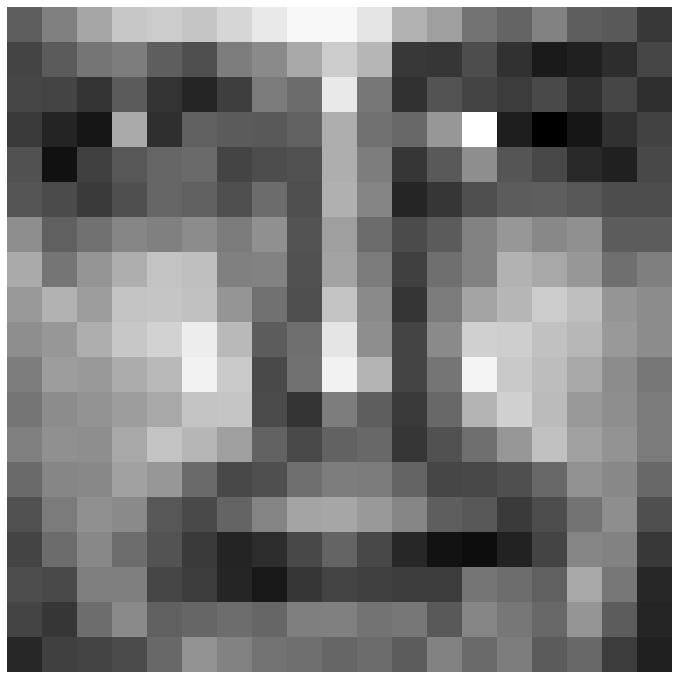
\includegraphics[width=0.3\linewidth]{PicturesResults/task1im.jpg}
    
\includegraphics[width=0.3\linewidth]{PicturesResults/task1ii_im.jpg}
    \caption{\texttt{im} \& \texttt{ii\_im}}
\end{figure}
\end{frame}

\begin{frame}
    \frametitle{Task I}
\begin{itemize}
\item \texttt{ComputeBoxSum}
\item \texttt{FeatureTypeI-IV}
    \debugpoint{2}
\item \texttt{EnumAllFeatures} 
\item \texttt{ComputeFeature}
    \debugpoint{3}
    \end{itemize}
\end{frame}

\begin{frame}
    \frametitle{Task I}
    \begin{itemize}
\item \texttt{VecBoxSum}
\item \texttt{VecFeature}
\item \texttt{VecAllFeatures}
\item \texttt{VecComputeFeatures}
\item \texttt{LoadSaveImData}
\item \texttt{ComputeSaveFData}
    \debugpoint{4}
\item \texttt{GetTrainingData}
    \debugpoint{5}
    \end{itemize}
\end{frame}

\section{Task II}

\begin{frame}
\frametitle{Task II}
\begin{itemize}
    \item \texttt{LearnWeakClassifier}
    \item \texttt{MakeFeaturePic}
    \item \texttt{MakeClassifierPic}
    \item \texttt{BoostingAlg}
        \debugpoint{6}
        \debugpoint{7}
\end{itemize}
\end{frame}

\begin{frame}
    \frametitle{Task II}
\begin{figure}
    \centering
    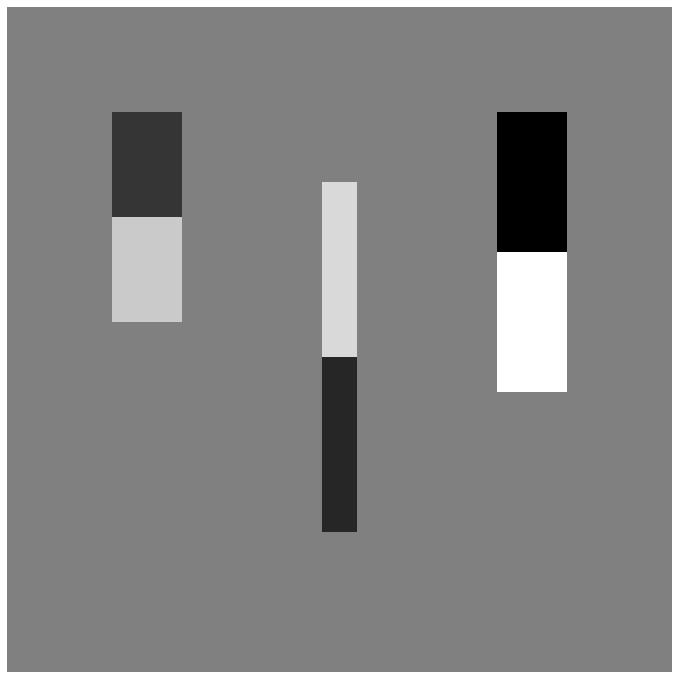
\includegraphics[width=0.3\linewidth]{PicturesResults/task2classifiers_debug6.jpg}
    
\includegraphics[width=0.3\linewidth]{PicturesResults/task2classifiers_debug7.jpg}
    \caption{Classifiers corresponding to debug 6 \& debug 7}
\end{figure}
\end{frame}

\section{Task III}

\begin{frame}
\frametitle{Task III}
\begin{itemize}
    \item \texttt{ApplyDetector}
    \item \texttt{ComputeRoc}
        \debugpoint{8}
\end{itemize}
\begin{figure}
    \centering
    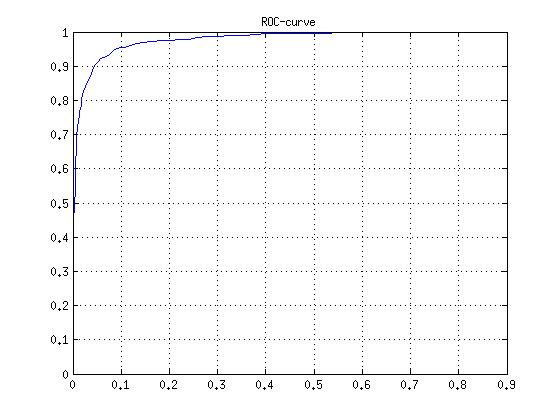
\includegraphics[width=0.4\linewidth]{PicturesResults/task3ROC.jpg}
    \caption{ROC-curve \\
    Threshold for 90\%: $5.11$}

\end{figure}

\end{frame}

\section{Task IV}

\begin{frame}
\frametitle{Task IV}
\begin{itemize}
    \item \texttt{ScanImageFixedSize}
    \item \texttt{DisplayDetections}
    \item \texttt{PruneDetections}
    \item \texttt{ScanImageOverScale}
        \debugpoint{9}
\end{itemize}
\end{frame}

\begin{frame}
\begin{figure}
    \centering
    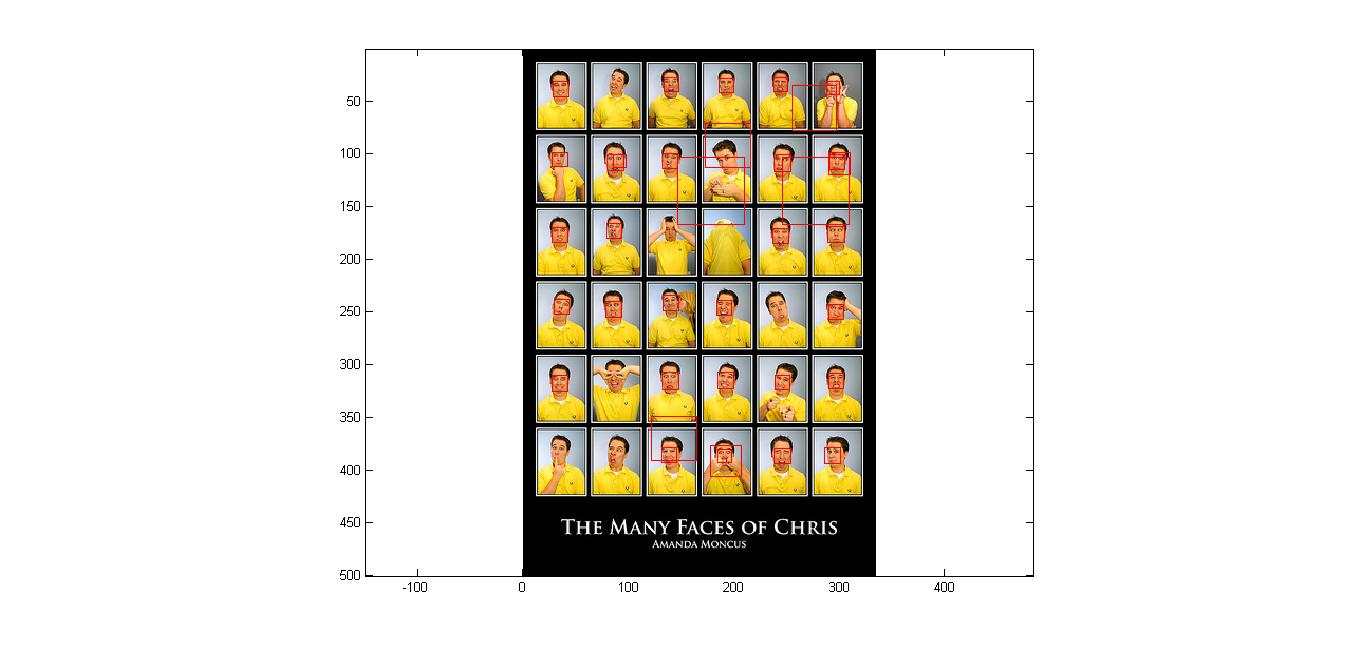
\includegraphics[height=0.5\linewidth]{PicturesResults/task4dets.jpg}
    \caption{Detection results}
\end{figure}
\end{frame}

\end{document}
